\section{Scalala}
\label{IMPL_SCALALA}
The DSL was implemented through the Scala GPL. However, this study should not give an introduction to Scala programming; rather, provide the DSL realisation through Scala as host language. Therefore, only the DSL relevant Scala features are emphasised and explained. The design process of a DSL was carefully evaluated and adopted from Mernik's et al. research.\cite{Mernik2005} He described five phases of DSL development and identified patterns in each phase. His patterns are not a guideline on how to implement a DSL in detail, instead of guiding the decision process. The subsections of this section are named and organised by Mernik's pattern-based implementation:

\begin{itemize}
\item Decision
\item Analysis
\item Design
\item Implementation
\item Deployment
\end{itemize}

The name \textit{Scalala} is adopted from the related project Scalala. It is a neologism, which consists of the GPL name \textit{Scala} and the onomatopoeia \textbf{la}. This onomatopoeia alludes to the \textbf{la-la} syllables in songs.

\subsection{Decision}
\label{IMPL_SCALALA_DECISION}
The related projects in section \ref{LIT_PROJ} already emphasised that there is no available programming language or holistic approach according to the thesis requirements defined in \ref{INTRO_SOFT}. Furthermore, the aim of this study is to \textit{create a user-friendly notation} and to \textit{transform} notes, which are usually described through visual sheet notes. In conclusion, these aspects map identically with Mernik's "Notation Pattern" and supports the decision to create a new "domain notation".\cite{Mernik2005}

To fulfil the results of Soloway's\cite{Soloway1982}  and Kranch's\cite{Kranch2012} research and create a novice-friendly programming language close to the natural language, the cardinality of external DSLs was used. In addition, external DSLs are more powerful and more flexible by nature (cf. \ref{THEO_DSL}).

\subsection{Analysis}
\label{IMPL_SCALALA_ANALYSIS}
Comprehensive analysis is necessary to create a fundamental groundwork for the DSL implementation. The target domain, or "problem domain" has to be carefully examined. The problem domain contains all major artefacts like processes, entities and constraints, which are part of the target business. The process is necessary to create a "common language" between domain expert and developer, to provide communication and prevent errors.\cite{Ghosh2010}

According to this, the "common vocabulary"\cite{Ghosh2010} or "common dictionary"\cite{Riti2018} was developed. An extract of the developed vocabulary is illustrated in table \ref{TBL_COMMONDICT}. Also, the common vocabulary was used to model the "solution domain" which provides all tools, to solve the present problem.\cite{Ghosh2010, Riti2018}

Figure \ref{IMG_DSL_DOMAINS} illustrates the relationships between all named domains and shows, how the common dictionary is used in both domains and acts as the "glue" between both.\cite{Ghosh2010} Even though this comprehensive process is fundamental work, Mernik classifies this process as the most used "Informal Analysis Pattern", since extensive studies or surveys with the target domain were not performed by this project.\cite{Mernik2005}

\begin{table}[h]
\caption{DSL Common Dictionary (truncated). All "Translations" are simplified.}
\label{TBL_COMMONDICT}
\begin{tabular}{l|p{200pt}|l}
\rowcolor{htwg-teal} 
\textbf{Problem Domain}      & \textbf{Translation}		& \textbf{Target Domain}     \\
full score                  						& Sheet music, which contains all instruments and voices. Arranged in a fixed order. 		& track \\
instruments /  voices 					& A specific instrument which is played by a specific person.							& musician \\
octave 											& 	An interval between two pitches.																						& octave \\
note													& combination of pitch and duration.																						& note (a-g) \\
. . .													& . . . 																																			& . . .
\end{tabular}
\end{table}

\begin{figure}[h]
\caption{Common Dictionary as Glue beteween Problem and Solution Domain.\cite[p. 15]{Ghosh2010}}
\label{IMG_DSL_DOMAINS}
\includegraphics[scale=0.5]{dsl_domains}
\end{figure}



\subsection{Design}
\label{IMPL_SCALALA_DESIGN}
As mentioned in the section before, part of designing a language is to create the solution domain. In this thesis, the solution domain was created by defining the language concepts and the basic DSL architecture. Since the approach is to create an external DSL, according to the "Language Invention" pattern, the language has to be developed from scratch. The automatic generation through modern language generation systems was not possible, because of the "informal" notation and characteristics.\cite{Mernik2005} The language was suitably designed to satisfy both domains:

\begin{itemize}
\item Developer Domain \newline According to Riti's suggestions, the architecture was developed to encapsulate and hide implementation details to reveal only the parts which are necessary to solve the problem. Further, the system was designed to be easily maintainable.\cite{Riti2018}

\item Novice Domain \newline As suggested by Kranch, the language was designed close to the natural language. The reason to design the language as close to the natural language as possible was that Kranch's researches with novices illustrate, that his subjects applied their knowledge from natural languages to make an analogy to the program elements.\cite{Kranch2012} Another requirement to the language was to teach fundamental programming concepts; like variable declaration/usage, basic arithmetic and method invocation.
\end{itemize}

Because of the absence of any precise definition in the literature, in which stage the final language grammar should be developed, in the design or in the implementation phase, the chosen approach was to define the grammar during the design phase. However, the grammar has to be designed decoupled of the final implementation.  This can be attributed to the grammar definition language—Extended Backus-Naur Form (EBNF)—which exists independently from any implementation or language in general. Listing \ref{LS_EBNF_TRUNC} highlights the root rule and the sub-rules.

\begin{lstlisting}[caption={EBNF (truncated).}, label=LS_EBNF_TRUNC]
(*** Terminals ***)
INSTRUMENT		::=	'instrument';
MUSICIAN		::=	'musician';
TEMPO			::=	'tempo';
WITH			::=	'with';
TEMPO			::=	'tempo';

STRING	::=	[a-z]+;
INT	::=	[0-9]+;


(*** Non-Terminals ***)
identifier	::=	STRING;
song		::=	(musician)* track;   
track		::=	PLAY (tempo)? musicVars;
tempo		::=	WITH TEMPO INT;
musicVars	::=	musicVar (COMMA musicVar)*;
	
. . .
\end{lstlisting}

\subsection{Implementation}
\label{IMPL_SCALALA_IMPL}
Mernik's "Interpreter" pattern was chosen to implement the DSL since the aim is to develop an external one; thus, it is necessary to provide a "fetch-decode-execute cycle". This cycle describes, in general, the input fetching through the lexer, decoding this input through the parser and the final translation into code. Besides, the advantages are simplicity, greater control over the execution environment and maintainability. The disadvantages, like the considerable effort to implement a complex language processor or the risk to end in an incoherent design, were found to be acceptable.\cite{Mernik2005}

The implementation process can be summarised as followed (cf. \cite{Ghosh2010}):

\begin{figure}[h]
\centering
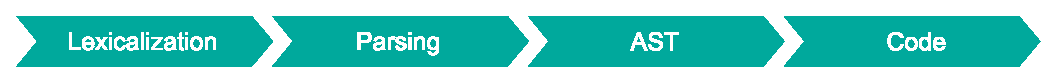
\includegraphics[scale=0.7]{impl_process_0}
\end{figure}

To be able to discuss each phase in more detail, the model is further divided into two layers:

\begin{itemize}
\item\textbf{1st Layer} Syntactic Analysis
\item\textbf{2nd Layer} Semantic Model
\end{itemize}

\subsubsection{Syntactic Analysis}
\label{IMPL_SCALALA_IMPL_SYNTACTIC}
The in EBNF notation modelled grammar was the starting point for the implementation. Based on this grammar, it is necessary to create the \textit{lexer}, also called \textit{tokeniser}, which handles the lexical analysis. The lexer splits an input stream into lexical units—the tokens. These tokens are the input of the parser. The parser generates a semantic model of the language and translates it into software.

The terms lexer and parser are often mixed and interchanged in the literature, since both have much in common. Moreover, a parser could act as the tokeniser for the next parser and so on. The main difference between both is the grammar:

\begin{itemize}
\item Lexer accepts regular grammars (Chomsky's level 3)
\item Parser accepts context-free grammars (Chomsky's level 2)\cite{Wagenknecht2014}
\end{itemize}

Due to the fact, that this study is not an introduction into language grammars, rather than in language design and implementation, the Chomsky hierarchy is not further explained. Wagenknecht et al. provides an overall introduction to language theory.\cite{Wagenknecht2014}

Depending on the complexity of the language, it could be a massive effort to create the lexer and the parser.\cite{Ghosh2010} This is one reason, why the DSL was developed through Scala; the Scala GPL offers the \textit{Parser Combinators} as a standard library which provides simple ways to create the abstraction model for the interpreter.

As an alternative to the parser combinators, it is possible to create the lexer \textbf{and} the parser through \textit{Parser Generators} like ANTLR\footnote{ANTLR - \url{http://www.antlr.org}}. The generators are tools with own configuration languages and settings.

\begin{figure}[h]
\centering
\includegraphics[scale=0.7]{impl_process_1}
\end{figure}

The lexer and parser were implemented in pure Scala, without any external tools or frameworks.\cite{Schmitt2014} Firstly the \textit{lexical parser} was developed to identify the lexing. The main idea behind the parser combinators is to define different parsers and \textit{combine} these to create one comprehensive parser.\cite{Riti2018} As mentioned before, lexing and parsing share many commonalities and are especially hard to isolate within the parser combinators; nevertheless, the lexer was implemented through extending the \texttt{StandardTokenParsers} class in according to Gosh and Riti.\cite{Ghosh2010, Riti2018} The lexer can be understood as the smallest parser unit. Through defining \textit{reserved} words and delimiters or using predefined parsers (like \texttt{numericLit} which defines numeric literal tokens), the lexer knows which chunk should be part of the input token stream. In the thesis's case, all reserved words were adopted from the EBNF terminal symbols. An extract of this lexer definition is illustrated in the listing \ref{LS_RESERVED_WORDS} below.

\begin{lstlisting}[caption={Defining the reserved words and delimiters through Scala's \texttt{StandardTokenParsers}}, label=LS_RESERVED_WORDS]
lexical.reserved += ("loop",
    "chord",
    "notes",
    "instrument",
    "musician",
    "with",
    "play",
    "plays",
    "tempo",
    "at",
    "c", "d", "e", "f", "g", "a", "h"
  lexical.delimiters += (",", "(", ")", "/", ".", "+", "-")
\end{lstlisting}

These predefined \textit{lexical parsers} are the groundwork for combining these parsers with other parsers.

\begin{figure}[h]
\centering
\includegraphics[scale=0.7]{impl_process_2}
\end{figure}

To apply the designed context-free grammar from \ref{IMPL_SCALALA_DESIGN}, Scala's parser combinators were utilised to define recursive descent (RD) parsers. RD parsers are the representation of \textit{recursive} functions to parse a tree starting at the top, ie. a top-down design (for further informations see Wagenknecht et al.\cite{Wagenknecht2014}). This parser is a direct implementation of a LL-parsers for LL(k)-grammars (usually $k = 1$).\cite{Ghosh2010}

The parser combinator offers the possibility to define a parser, which looks like an EBNF and its production rules. This is also the place where Scala proved to be very usefull since the parsers could be implemented with higher-order functions. This circumstance reduces redundant code considerably and provides the creation of small parser parts, each decoupled from another and composes them functionally to generate one large parser. Listing \ref{LS_PARSER_INIT} illustrates the first production rules which represent the initial parser rule (simplified). The names were adopted directly from the predefined EBNF; it is essential to apply this names, as suggested by Gosh because the rules reflect the domain concept and the "blueprint" to communicate with the domain experts.\cite{Ghosh2010}

\begin{lstlisting}[caption={Initial parser combinator rules. (simplified)}, label=LS_PARSER_INIT]
lazy val song		=	rep(musician) ~ track

lazy val musician	=	"musician" ~> ident

lazy val track		=	"play" ~> repsep(musician, ",")
\end{lstlisting}

The defined parser \texttt{song} already consists of two further parsers, \texttt{musician} and \texttt{track}, each of them represents a combination of further parsers, and so on. The elements are described as follows:

\begin{itemize}
\item\texttt{rep(musician)} \newline Repeats  \texttt{musician}   one or more times.
\item\texttt{repsep(musician, ",")} \newline Repeats  \texttt{musician}   one or more times with the separator  \texttt{","}.
\item\texttt{"musician"} \newline Represents a  \texttt{keyword}   which was defined at the  \texttt{lexicalization}   (cf. Lexicalization) and is parsed through the  \texttt{lexer parser}.
\item\texttt{"play"} \newline Same as  \texttt{"musician" }.
\item\texttt{ident} \newline Also a lexer representation which matches an identifier (String).
\end{itemize}

Each parser, like \texttt{rep(musician)} or \texttt{track}, composes a DSL syntax parser sequentially. To combine each of them, \textit{combinators} are applied (represented as higher order functions). Combinators are represented through symbols for brevity and implemented as methods within the Scala class \texttt{Parsers[T]}.\cite{Ghosh2010}

Presumed \texttt{P} and \texttt{Q} are parsers, they can be combined as shown in table \ref{TBL_COMBINATORS}. Note, however, that this table represents only the common productions rules, and is not complete.

\begin{table}[h]
\caption{Scala Parsers (truncated).\cite{Riti2018}}
\label{TBL_COMBINATORS}
\begin{tabular}{l|l|p{180pt}}
\rowcolor{htwg-teal} 
\textbf{Parser}      & \textbf{Name}		& \textbf{Description}     \\
\lstinline|P ~ Q|						& Sequence 					& \texttt{P} consumes the first part of the input stream, followed by \texttt{Q}, which consumes the remaining part from \texttt{P}. \\
\lstinline|P ~> Q|		 					& Selective Sequence	& Works like \lstinline|~|, but returns only the result from \texttt{} Q. However, \texttt{P}'s presence is necessary but can be dropped from the result. \\
\texttt{P | Q}								& Alternation					& Acts identically to the EBNF \texttt{|} symbol which represents an \texttt{OR} connection between two parsers.
\end{tabular}
\end{table}

To transform an input into a result, each parser implements the methods \texttt{Success}, \texttt{Failure} and \texttt{Error}. This allows the parser to use \textit{backtracking}. For example, the parser combinator \lstinline|P ~ Q| can be explained as follows (cf. \cite{Ghosh2010}):

\begin{itemize}
\item If \texttt{P} ends in \texttt{Success} then, and only then, \texttt{Q} is examined and is fed with the truncated input stream.

\item If \texttt{P} ends in \texttt{Failure}, the input stream can not be matched with this parser, \texttt{Q} is not further examined and, backtracking is invoked to try alternative rules—if there are any available.

\item If \texttt{Failure} is fatal or another runtime exception happens, \texttt{Failure} ends in \texttt{Error}, no backtracking is done, and the process returns.
\end{itemize}

This short example, as well as table \ref{TBL_COMBINATORS} and listing \ref{LS_PARSER_INIT}, however, disclose already the disadvantage \textbf{and} advantage of Scala's parser combinator: the short syntax and its accompanying readability.

The combinator symbols utilize another Scala feature, called infix operation notation, and are predefined methods within the class \texttt{Parsers[T]}. If the infix notation is suppressed, the sequence combinator \lstinline|P ~ Q| would be a simple method call \lstinline|P.~(Q)|. This notation allows exact and short code and to model the parser similar to the EBNF notation.\cite{Ghosh2010}

The parser represents the DSL's core junction between the designed language through EBNF notation and the programming language. To create the AST, the current layer \textit{Syntactic Analyse} is left, and the further steps are explained in the following layer—\textit{Semantic Model}.

\subsubsection{Semantic Model}
\label{IMPL_SCALALA_IMPL_SEMANTIC}

\begin{figure}[h]
\centering
\includegraphics[scale=0.7]{impl_process_3}
\end{figure}

The essential part to create the connection between the parsed structure, the grammar and the final output, is to generate the semantic model in memory which is the actual result of the parser. The semantic model is usually an AST. Each node in the tree represents a token which is used in the grammar. Using the method of Riti, a homogenous AST was implemented, since it is the most straightforward approach to walk through the AST and generate the final code.\cite{Riti2018}

To create this tree, the implemented parser was extended to transform the result of a particular parser in such way that the semantic model is built incrementally. Through \textit{function application combinators} the parser applies functions to the parsed input stream. Listing \ref{LS_PARSER_FUNC} illustrates the extended version of listing \ref{LS_PARSER_INIT} with \textit{function application}.

\begin{lstlisting}[caption={Parser combinator rules extended through \textit{function application}.}, label=LS_PARSER_FUNC]
lazy val song: Parser[Song] = rep(musician) ~ track ^^ {
	case m ~ t => Song(m, t)
}

lazy val musician: Parser[Musician] = "musician" ~> ident ^^ {
	case m => Musician(m)
}

lazy val track: Parser[Track] = "play" ~> repsep(musician, ",") ^^ {
	case m => Track(m)
}
\end{lstlisting}

Again, the symbol \lstinline|^^| is just a method call, shortened through infix notation.\cite{Ghosh2010} The return value of an applied function matches the defined return value from the parsers signature (implicit). Scala's \textit{case classes} functionality directly supports the AST creation by matching the succeeded parser and assigning the matched values to an object. However, to create the AST representation as described, the underlying semantic model has to be predefined. Simplified, the semantic model is just plain Scala and represents all traits, case classes and objects which are in use. Finally, the AST is the result from the parser itself and allows the translator to \textit{walk} through all objects and create the output.


\begin{figure}[h]
\centering
\includegraphics[scale=0.7]{impl_process_4}
\end{figure}

The final output generation is the last step in converting an input DSL script into code and is handled by the interpreter. In the thesis's case, the output is the MIDI sound file. To convert the AST in actual output, the \textit{tree-pattern-matcher} was used.\cite{Riti2018} The AST is walked through recursively, and through pattern matching, an action is invoked at the relevant term. The graphical representation of this \textit{process} is the translation result of the input DSL script example in listing \ref{LS_DSL_WALK} and is illustrated in figure \ref{IMG_DSL_AST}. The MIDI generation is explained in section \ref{IMPL_SCALALA_MIDI}.

\begin{lstlisting}[caption={DSL script example.}, label=LS_DSL_WALK]
musician pianist_1
   instrument Piano
   plays c,d,e

play with tempo 60
   pianist_1
\end{lstlisting}

\begin{figure}[h]
\caption{DSL script example - AST.}
\label{IMG_DSL_AST}
\includegraphics[scale=0.57]{ast}
\end{figure}





\subsection{Deployment}
\label{IMPL_SCALALA_DEPL}
In this study, the DSL was deployed as a Scala library. Thus, an easy to apply deployment mechanism to continuous integration tools like \textit{Travis-CI} is possible and the integration into other applications is straightforward.
\newline
\newline
This section illustrated, how the DSL was designed from scratch and implemented by the Scala parser combinator. To conclude, Mernik's decisions guideline\cite{Mernik2005} through patterns provided an excellent basic structure in DSL development. The Scala parser combinators are a reliable approach to implement an external DSL. Through functional programming and pattern matching, an abstraction of the defined grammar was easy to implement. However, since there is no official comprehensive documentation for Scala's parser combinator, it was very time-consuming to become familiar with the library and achieve results.


\subsection{MIDI}
\label{IMPL_SCALALA_MIDI}
In addition to the \textit{code generation} part of the DSL implementation, the interpreter was also implemented as the generator of the sound result. As already mentioned before, the DSL was implemented on top of the related project Scalala, which already provides the necessary MIDI representation. For the sake of simplicity, some parts of the semantic model rely on the Scalala model and were reused. Since Scalala represents an internal DSL, the implemented external DSL was developed on top of the internal one, which is a frequently used approach in the literature (cf. \cite{Fowler2010}).

While the interpreter is \textit{walking} through the AST recursively, the MIDI representation is constructed incrementally. The MIDI generation process was implemented as a plain Scala class which builds up the basic MIDI file structure and provides public methods to add notes, switch the instrument, set the tempo, etc. The implementation was done according to the MIDI-standard description.\cite{MIDIManufacturersAssociation} As in \ref{THEO_MIDI} described, the MIDI-protocol is constructed through byte-data sets and messages. This approach offers a fully flexible way to create MIDI-sound-files. However, the implementation, as well as the debugging at the byte-level, is less than ideal. Since the MIDI-file represents a binary file, it is not possible to comprehend which sequences were written to the file; a third-party application is necessary to decode the file, examine its contents and verify the correctness. In the thesis's case, the MacOS application \textit{MidiMusicXmlPlayer}\footnote{MidiMusicXmlPlayer v1.60 - \url{http://programfabriken.com}} was used and provided excellent results in MIDI decoding and playback.













